% Practice Test 08 — Oklahoma Edition
% Questions: 30 (21 MC + 9 SA)
% Generated by scripts/generate_practice_tests.py

\begin{practiceQuestion}{1-3-q13}{mc}
\begin{questionText}
The table shows a proportional relationship. Find the missing value.

\begin{center}
\begin{tabular}{|c|c|}
\hline $x$ & $y$ \\ \hline $4$ & $14$ \\ $6$ & $?$ \\ $10$ & $35$ \\ \hline
\end{tabular}
\end{center}
\end{questionText}
\choiceA{$18$}
\choiceB{$20$}
\choiceC{$21$}
\choiceD{$24$}
\correctAnswer{C}
\explanation{$k = \frac{14}{4} = 3.5$. Missing value: $y = 3.5 \times 6 = 21$. Check: $\frac{35}{10} = 3.5$ \checkmark.}
\end{practiceQuestion}

\begin{practiceQuestion}{1-6-q21}{sa}
\begin{questionText}
A scale drawing uses $1$ cm $= 4.5$ m. If a building is $27$ m tall, how tall is it in the drawing?
\end{questionText}
\correctAnswer{$6$ cm}
\explanation{$\frac{1}{4.5} = \frac{x}{27}$. Cross-multiply: $4.5x = 27$, so $x = 6$ cm.}
\end{practiceQuestion}

\begin{practiceQuestion}{1-7-q26}{gmc}
\begin{questionText}
The diagram below shows a model building and its actual building. The model is $6$ cm tall. The scale is $1 : 150$. Which label correctly shows the actual height?

\begin{center}
\begin{tikzpicture}[scale=0.8]
  % Model building
  \draw[thick,funBlue,fill=funBlue!20] (0,0) rectangle (1,1.5);
  \node[below] at (0.5,0) {Model};
  \draw[<->] (-0.3,0) -- (-0.3,1.5) node[midway,left] {$6$ cm};

  % Arrow
  \draw[thick,->] (1.8,0.75) -- (3.2,0.75) node[midway,above] {$\times\;150$};

  % Actual building
  \draw[thick,funRed,fill=funRed!20] (4,0) rectangle (5.5,3.5);
  \node[below] at (4.75,0) {Actual};
  \draw[<->] (5.8,0) -- (5.8,3.5) node[midway,right] {?};
\end{tikzpicture}
\end{center}
\end{questionText}
\choiceA{$90$ m}
\choiceB{$9$ m}
\choiceC{$900$ m}
\choiceD{$0.9$ m}
\correctAnswer{B}
\explanation{Multiply: $6 \times 150 = 900$ cm $= 9$ m.}
\end{practiceQuestion}

\begin{practiceQuestion}{2-1-q10}{mc}
\begin{questionText}
What is $8\%$ of $250$?
\end{questionText}
\choiceA{$2$}
\choiceB{$16$}
\choiceC{$20$}
\choiceD{$32$}
\correctAnswer{C}
\explanation{$8\% = 0.08$. Multiply: $0.08 \times 250 = 20$.}
\end{practiceQuestion}

\begin{practiceQuestion}{2-4-q17}{mc}
\begin{questionText}
A coat originally costs $\$85$. It goes on clearance for $40\%$ off, then an additional $10\%$ off the sale price. What is the final price before tax?
\end{questionText}
\choiceA{$\$42.50$}
\choiceB{$\$45.90$}
\choiceC{$\$51.00$}
\choiceD{$\$55.25$}
\correctAnswer{B}
\explanation{First discount: $85 \times 0.60 = \$51$. Second discount: $51 \times 0.90 = \$45.90$.}
\end{practiceQuestion}

\begin{practiceQuestion}{2-7-q27}{gmc}
\begin{questionText}
The bar graph shows the estimated and actual heights of three trees. Which tree has the greatest percent error?

\begin{center}
\begin{tikzpicture}[scale=0.5]
  \draw[thick,->] (0,0) -- (0,7) node[above]{\small Height (ft)};
  \draw[thick,->] (0,0) -- (10.5,0);
  % Tree A: est 20, actual 25
  \fill[funBlue!60] (0.5,0) rectangle (1.5,4);
  \fill[funGreen!60] (1.5,0) rectangle (2.5,5);
  % Tree B: est 15, actual 12
  \fill[funBlue!60] (3.5,0) rectangle (4.5,3);
  \fill[funGreen!60] (4.5,0) rectangle (5.5,2.4);
  % Tree C: est 30, actual 28
  \fill[funBlue!60] (6.5,0) rectangle (7.5,6);
  \fill[funGreen!60] (7.5,0) rectangle (8.5,5.6);
  % Labels
  \node[below,font=\small] at (1.5,0) {Tree A};
  \node[below,font=\small] at (4.5,0) {Tree B};
  \node[below,font=\small] at (7.5,0) {Tree C};
  \foreach \y/\lab in {1/5,2/10,3/15,4/20,5/25,6/30} {
    \draw (-0.1,\y) -- (0.1,\y) node[left,font=\small,xshift=-2pt] {\lab};
  }
  % Values
  \node[above,font=\scriptsize,funBlue] at (1,4) {$20$};
  \node[above,font=\scriptsize,funGreen!80!black] at (2,5) {$25$};
  \node[above,font=\scriptsize,funBlue] at (4,3) {$15$};
  \node[above,font=\scriptsize,funGreen!80!black] at (5,2.4) {$12$};
  \node[above,font=\scriptsize,funBlue] at (7,6) {$30$};
  \node[above,font=\scriptsize,funGreen!80!black] at (8,5.6) {$28$};
  % Legend
  \fill[funBlue!60] (0.5,6.8) rectangle (1,7.2);
  \node[right,font=\scriptsize] at (1.1,7) {Estimated};
  \fill[funGreen!60] (3.5,6.8) rectangle (4,7.2);
  \node[right,font=\scriptsize] at (4.1,7) {Actual};
\end{tikzpicture}
\end{center}
\end{questionText}
\choiceA{Tree A ($20\%$)}
\choiceB{Tree B ($25\%$)}
\choiceC{Tree C ($7.1\%$)}
\choiceD{Trees A and B are tied}
\correctAnswer{B}
\explanation{A: $|20-25|/25 = 20\%$. B: $|15-12|/12 = 25\%$. C: $|30-28|/28 \approx 7.1\%$. Tree B has the greatest error.}
\end{practiceQuestion}

\begin{practiceQuestion}{2-8-q04}{mc}
\begin{questionText}
You buy a $\$500$ laptop using a credit card at $12\%$ annual interest. If you pay it all back after $1$ year, what is the total cost?
\end{questionText}
\choiceA{$\$512$}
\choiceB{$\$560$}
\choiceC{$\$600$}
\choiceD{$\$550$}
\correctAnswer{B}
\explanation{Interest $= 500 \times 0.12 \times 1 = \$60$. Total $= 500 + 60 = \$560$.}
\end{practiceQuestion}

\begin{practiceQuestion}{3-1-q12}{mc}
\begin{questionText}
The temperature at noon was $5°$C. By midnight it was $-5°$C. What is the relationship between these temperatures?
\end{questionText}
\choiceA{They are equal}
\choiceB{They are opposites}
\choiceC{Midnight was warmer}
\choiceD{Their absolute values are different}
\correctAnswer{B}
\explanation{$5$ and $-5$ are the same distance from $0$ but on opposite sides of the number line. They are opposites.}
\end{practiceQuestion}

\begin{practiceQuestion}{4-1-q25}{sa}
\begin{questionText}
A student earns $\$8.50$ per hour at a part-time job. Write an expression for the weekly earnings if the student works $h$ hours, and find the earnings for a $20$-hour week.
\end{questionText}
\correctAnswer{$8.50h$; $\$170$}
\explanation{Weekly earnings: $8.50h$. For $h = 20$: $8.50(20) = \$170$.}
\end{practiceQuestion}

\begin{practiceQuestion}{4-2-q03}{mc}
\begin{questionText}
Simplify $9a - 4a + 6$.
\end{questionText}
\choiceA{$11a$}
\choiceB{$5a + 6$}
\choiceC{$5a - 6$}
\choiceD{$13a - 4$}
\correctAnswer{B}
\explanation{Combine $9a - 4a = 5a$. The constant $6$ stays. Result: $5a + 6$.}
\end{practiceQuestion}

\begin{practiceQuestion}{5-3-q30}{gsa}
\begin{questionText}
Four friends go to a museum. Each person pays for a ticket and a $\$3$ audio guide. The total for all four people is $\$68$. The equation $4(t + 3) = 68$ represents this situation, where $t$ is the ticket price. Use the model below to find $t$.

\begin{center}
\begin{tikzpicture}[scale=0.6]
  % 4 bars
  \foreach \i in {0,...,3} {
    \draw[thick,fill=funBlue!20] (0,\i*1.2) rectangle (6,\i*1.2+0.9);
    \draw[thick,fill=funOrange!30] (6,\i*1.2) rectangle (8,\i*1.2+0.9);
    \node at (3,\i*1.2+0.45) {$t$};
    \node at (7,\i*1.2+0.45) {$\$3$};
  }
  \node[left] at (-0.3,1.8) {$4$ people};
  \draw[decorate,decoration={brace,amplitude=6pt}] (8.3,4.5) -- (8.3,0);
  \node[right] at (8.7,2.25) {$\$68$};
\end{tikzpicture}
\end{center}
\end{questionText}
\correctAnswer{$t = \$14$}
\explanation{$4(t + 3) = 68$. Divide by $4$: $t + 3 = 17$. Subtract $3$: $t = 14$. Each ticket costs $\$14$.}
\end{practiceQuestion}

\begin{practiceQuestion}{5-4-q19}{sa}
\begin{questionText}
Solve $\dfrac{3x}{4} - 2 = 7$.
\end{questionText}
\correctAnswer{$x = 12$}
\explanation{Add $2$: $\frac{3x}{4} = 9$. Multiply by $4$: $3x = 36$. Divide by $3$: $x = 12$. Check: $\frac{3(12)}{4} - 2 = 9 - 2 = 7$ \checkmark.}
\end{practiceQuestion}

\begin{practiceQuestion}{5-5-q21}{sa}
\begin{questionText}
Write an inequality: ``A number $x$ divided by $4$, minus $3$, is at least $2$.'' Then solve.
\end{questionText}
\correctAnswer{$\dfrac{x}{4} - 3 \geq 2$; $x \geq 20$}
\explanation{$\frac{x}{4} - 3 \geq 2$. Add $3$: $\frac{x}{4} \geq 5$. Multiply by $4$: $x \geq 20$.}
\end{practiceQuestion}

\begin{practiceQuestion}{5-6-q07}{mc}
\begin{questionText}
The graph of an inequality has an open circle at $-1$ and is shaded to the left. Which inequality matches?
\end{questionText}
\choiceA{$x \leq -1$}
\choiceB{$x < -1$}
\choiceC{$x \geq -1$}
\choiceD{$x > -1$}
\correctAnswer{B}
\explanation{Open circle means $-1$ is not included, shading left means less than: $x < -1$.}
\end{practiceQuestion}

\begin{practiceQuestion}{6-2-q02}{mc}
\begin{questionText}
A blueprint uses $1$ cm $= 4$ m. You want to redraw it at $1$ cm $= 8$ m. A wall that is $10$ cm on the original becomes how long on the new drawing?
\end{questionText}
\choiceA{$5$ cm}
\choiceB{$10$ cm}
\choiceC{$20$ cm}
\choiceD{$40$ cm}
\correctAnswer{A}
\explanation{Scale ratio: $\frac{4}{8} = \frac{1}{2}$. New length: $10 \times \frac{1}{2} = 5$ cm. A larger scale (more real units per cm) shrinks the drawing.}
\end{practiceQuestion}

\begin{practiceQuestion}{6-3-q24}{sa}
\begin{questionText}
You are given angles $45°$ and $45°$ and side $6$ cm between them. How many triangles can you draw?
\end{questionText}
\correctAnswer{Exactly one}
\explanation{ASA (two angles and the included side) fully determine a unique triangle. The third angle would be $180° - 45° - 45° = 90°$.}
\end{practiceQuestion}

\begin{practiceQuestion}{6-4-q28}{gmc}
\begin{questionText}
The diagram shows two triangles. Both have angles $30°$, $60°$, and $90°$, but different side lengths. What does this demonstrate?

\begin{center}
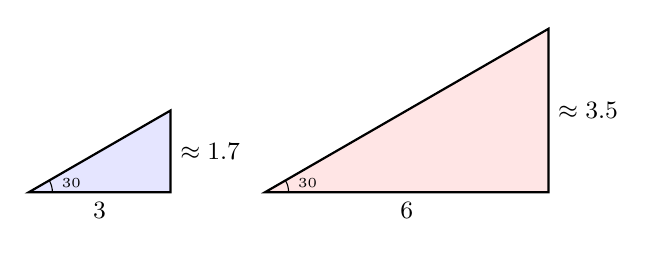
\begin{tikzpicture}[scale=0.6]
  % Small triangle
  \draw[thick,fill=blue!10] (0,0) -- (3,0) -- (3,1.73) -- cycle;
  \node[below] at (1.5,0) {\small $3$};
  \node[right] at (3,0.86) {\small $\approx 1.7$};
  \draw (0.5,0) arc[start angle=0,end angle=30,radius=0.5];
  \node at (0.9,0.2) {\tiny $30°$};
  % Large triangle
  \draw[thick,fill=red!10] (5,0) -- (11,0) -- (11,3.46) -- cycle;
  \node[below] at (8,0) {\small $6$};
  \node[right] at (11,1.73) {\small $\approx 3.5$};
  \draw (5.5,0) arc[start angle=0,end angle=30,radius=0.5];
  \node at (5.9,0.2) {\tiny $30°$};
\end{tikzpicture}
\end{center}
\end{questionText}
\choiceA{SSS produces multiple triangles}
\choiceB{AAA produces a unique triangle}
\choiceC{AAA produces multiple triangles of different sizes}
\choiceD{These two triangles are congruent}
\correctAnswer{C}
\explanation{Both triangles have the same angles but different side lengths. AAA determines shape but not size, so many triangles are possible.}
\end{practiceQuestion}

\begin{practiceQuestion}{6-5-q15}{mc}
\begin{questionText}
A pyramid with a square base is sliced with a horizontal cut near the top. What shape is the cross-section?
\end{questionText}
\choiceA{A very small square}
\choiceB{A triangle}
\choiceC{A point}
\choiceD{A circle}
\correctAnswer{A}
\explanation{A horizontal cut of a square pyramid parallel to the base gives a square. Near the top, the square is very small. At the very apex it would be a point, but a cut ``near the top'' gives a small square.}
\end{practiceQuestion}

\begin{practiceQuestion}{6-6-q04}{mc}
\begin{questionText}
Two supplementary angles are $(2x + 10)°$ and $(3x)°$. What is the value of $x$?
\end{questionText}
\choiceA{$30$}
\choiceB{$34$}
\choiceC{$36$}
\choiceD{$40$}
\correctAnswer{B}
\explanation{$2x + 10 + 3x = 180$. Combine: $5x + 10 = 180$. Subtract $10$: $5x = 170$. Divide: $x = 34$.}
\end{practiceQuestion}

\begin{practiceQuestion}{7-4-q17}{mc}
\begin{questionText}
A swimming pool is shaped like a rectangle $25$ m by $10$ m with a semicircle of diameter $10$ m at one end. What is the total area? Use $\pi \approx 3.14$.
\end{questionText}
\choiceA{$250$ m$^2$}
\choiceB{$289.25$ m$^2$}
\choiceC{$328.5$ m$^2$}
\choiceD{$367.75$ m$^2$}
\correctAnswer{B}
\explanation{Rectangle: $25 \times 10 = 250$ m$^2$. Semicircle: $\frac{1}{2} \times 3.14 \times 5^2 = \frac{1}{2} \times 78.5 = 39.25$ m$^2$. Total: $250 + 39.25 = 289.25$ m$^2$.}
\end{practiceQuestion}

\begin{practiceQuestion}{7-5-q26}{gmc}
\begin{questionText}
The net of a rectangular prism is shown below. What is the total surface area?

\begin{center}
\begin{tikzpicture}[scale=0.4]
  % Base cross-shaped net
  \draw[thick,funBlue,fill=funBlue!10] (0,0) rectangle (6,4);
  \node at (3,2) {$6 \times 4$};
  \draw[thick,funBlue,fill=funBlue!10] (6,0) rectangle (9,4);
  \node at (7.5,2) {$3 \times 4$};
  \draw[thick,funBlue,fill=funBlue!10] (9,0) rectangle (15,4);
  \node at (12,2) {$6 \times 4$};
  \draw[thick,funBlue,fill=funBlue!10] (15,0) rectangle (18,4);
  \node at (16.5,2) {$3 \times 4$};
  \draw[thick,funBlue,fill=funBlue!10] (0,4) rectangle (6,7);
  \node at (3,5.5) {$6 \times 3$};
  \draw[thick,funBlue,fill=funBlue!10] (0,-3) rectangle (6,0);
  \node at (3,-1.5) {$6 \times 3$};
\end{tikzpicture}
\end{center}
\end{questionText}
\choiceA{$72$ square units}
\choiceB{$84$ square units}
\choiceC{$108$ square units}
\choiceD{$144$ square units}
\correctAnswer{C}
\explanation{Two $6 \times 4$ faces: $48$. Two $3 \times 4$ faces: $24$. Two $6 \times 3$ faces: $36$. Total: $48 + 24 + 36 = 108$ square units.}
\end{practiceQuestion}

\begin{practiceQuestion}{7-6-q20}{sa}
\begin{questionText}
A cube has a side length of $6$ inches. What is its volume?
\end{questionText}
\correctAnswer{$216$ in$^3$}
\explanation{$V = 6^3 = 216$ in$^3$.}
\end{practiceQuestion}

\begin{practiceQuestion}{8-1-q16}{mc}
\begin{questionText}
Why is a convenience sample (e.g., surveying your friends) usually not a good way to learn about a population?
\end{questionText}
\choiceA{It is too expensive}
\choiceB{It takes too long}
\choiceC{It is likely biased and not representative}
\choiceD{It includes too many people}
\correctAnswer{C}
\explanation{Convenience samples are easy but likely biased because they don't give everyone an equal chance.}
\end{practiceQuestion}

\begin{practiceQuestion}{8-3-q30}{gsa}
\begin{questionText}
The dot plots show quiz scores for two classes (out of $10$).

\begin{center}
\begin{tikzpicture}[scale=0.6]
  % Class X
  \node[left,font=\small\bfseries] at (3.5,2) {Class X};
  \draw[thick,->] (3.5,0) -- (11.5,0);
  \foreach \x in {4,5,...,10} {
    \draw (\x,0.1) -- (\x,-0.1);
    \node[below,font=\small] at (\x,0) {$\x$};
  }
  % Class X data: 5(1),6(2),7(4),8(5),9(3),10(1) = 16 students
  \fill[funBlue] (5,0.35) circle (0.13);
  \fill[funBlue] (6,0.35) circle (0.13); \fill[funBlue] (6,0.65) circle (0.13);
  \fill[funBlue] (7,0.35) circle (0.13); \fill[funBlue] (7,0.65) circle (0.13); \fill[funBlue] (7,0.95) circle (0.13); \fill[funBlue] (7,1.25) circle (0.13);
  \fill[funBlue] (8,0.35) circle (0.13); \fill[funBlue] (8,0.65) circle (0.13); \fill[funBlue] (8,0.95) circle (0.13); \fill[funBlue] (8,1.25) circle (0.13); \fill[funBlue] (8,1.55) circle (0.13);
  \fill[funBlue] (9,0.35) circle (0.13); \fill[funBlue] (9,0.65) circle (0.13); \fill[funBlue] (9,0.95) circle (0.13);
  \fill[funBlue] (10,0.35) circle (0.13);

  % Class Y
  \node[left,font=\small\bfseries] at (3.5,5.5) {Class Y};
  \draw[thick,->] (3.5,3.5) -- (11.5,3.5);
  \foreach \x in {4,5,...,10} {
    \draw (\x,3.6) -- (\x,3.4);
  }
  % Class Y data: 4(2),5(3),6(4),7(3),8(2),9(1),10(1) = 16 students
  \fill[funGreen] (4,3.85) circle (0.13); \fill[funGreen] (4,4.15) circle (0.13);
  \fill[funGreen] (5,3.85) circle (0.13); \fill[funGreen] (5,4.15) circle (0.13); \fill[funGreen] (5,4.45) circle (0.13);
  \fill[funGreen] (6,3.85) circle (0.13); \fill[funGreen] (6,4.15) circle (0.13); \fill[funGreen] (6,4.45) circle (0.13); \fill[funGreen] (6,4.75) circle (0.13);
  \fill[funGreen] (7,3.85) circle (0.13); \fill[funGreen] (7,4.15) circle (0.13); \fill[funGreen] (7,4.45) circle (0.13);
  \fill[funGreen] (8,3.85) circle (0.13); \fill[funGreen] (8,4.15) circle (0.13);
  \fill[funGreen] (9,3.85) circle (0.13);
  \fill[funGreen] (10,3.85) circle (0.13);
\end{tikzpicture}
\end{center}

Find the mean score for each class and determine which class performed better on the quiz.
\end{questionText}
\correctAnswer{Class X mean $\approx 7.75$; Class Y mean $\approx 6.25$. Class X performed better.}
\explanation{Class X: $(5+12+28+40+27+10) \div 16 = 122 \div 16 \approx 7.63$. Class Y: $(8+15+24+21+16+9+10) \div 16 = 103 \div 16 \approx 6.44$. Class X has a higher mean.}
\end{practiceQuestion}

\begin{practiceQuestion}{8-4-q01}{mc}
\begin{questionText}
Data set A: $10, 12, 14, 16, 18$. What is the mean?
\end{questionText}
\choiceA{$12$}
\choiceB{$14$}
\choiceC{$16$}
\choiceD{$70$}
\correctAnswer{B}
\explanation{$\frac{10+12+14+16+18}{5} = \frac{70}{5} = 14$.}
\end{practiceQuestion}

\begin{practiceQuestion}{8-5-q14}{mc}
\begin{questionText}
A back-to-back stem-and-leaf plot is used to:
\end{questionText}
\choiceA{Show one data set with two stems}
\choiceB{Compare two data sets using the same stems}
\choiceC{Display data that has been doubled}
\choiceD{Show data in a circle}
\correctAnswer{B}
\explanation{A back-to-back plot has leaves for one group on the left and for another group on the right, sharing the same stems.}
\end{practiceQuestion}

\begin{practiceQuestion}{8-7-q03}{mc}
\begin{questionText}
A double bar graph is used to:
\end{questionText}
\choiceA{Show one data set over time}
\choiceB{Compare two data sets using side-by-side bars}
\choiceC{Show parts of a whole}
\choiceD{Display individual data points}
\correctAnswer{B}
\explanation{Double bar graphs place two sets of bars side by side for each category so you can compare them directly.}
\end{practiceQuestion}

\begin{practiceQuestion}{9-4-q21}{sa}
\begin{questionText}
A bag has $6$ red, $4$ blue, and $10$ white marbles. Write the probability model by listing $P(\text{red})$, $P(\text{blue})$, and $P(\text{white})$ as fractions in simplest form.
\end{questionText}
\correctAnswer{$P(\text{red}) = \frac{3}{10}$, $P(\text{blue}) = \frac{1}{5}$, $P(\text{white}) = \frac{1}{2}$}
\explanation{Total: $20$. $P(\text{red}) = \frac{6}{20} = \frac{3}{10}$, $P(\text{blue}) = \frac{4}{20} = \frac{1}{5}$, $P(\text{white}) = \frac{10}{20} = \frac{1}{2}$.}
\end{practiceQuestion}

\begin{practiceQuestion}{9-6-q26}{gmc}
\begin{questionText}
The table shows all possible sums when two dice are rolled. What is the probability of rolling a sum of $8$?

\begin{center}
\begin{tabular}{|c|c|c|c|c|c|c|}
\hline
$+$ & \textbf{1} & \textbf{2} & \textbf{3} & \textbf{4} & \textbf{5} & \textbf{6} \\
\hline
\textbf{1} & $2$ & $3$ & $4$ & $5$ & $6$ & $7$ \\
\hline
\textbf{2} & $3$ & $4$ & $5$ & $6$ & $7$ & \cellcolor{funBlue!20}$8$ \\
\hline
\textbf{3} & $4$ & $5$ & $6$ & $7$ & \cellcolor{funBlue!20}$8$ & $9$ \\
\hline
\textbf{4} & $5$ & $6$ & $7$ & \cellcolor{funBlue!20}$8$ & $9$ & $10$ \\
\hline
\textbf{5} & $6$ & $7$ & \cellcolor{funBlue!20}$8$ & $9$ & $10$ & $11$ \\
\hline
\textbf{6} & $7$ & \cellcolor{funBlue!20}$8$ & $9$ & $10$ & $11$ & $12$ \\
\hline
\end{tabular}
\end{center}
\end{questionText}
\choiceA{$\frac{4}{36}$}
\choiceB{$\frac{5}{36}$}
\choiceC{$\frac{6}{36}$}
\choiceD{$\frac{8}{36}$}
\correctAnswer{B}
\explanation{Outcomes with sum $8$: $(2,6), (3,5), (4,4), (5,3), (6,2)$ — that is $5$. $P = \frac{5}{36}$.}
\end{practiceQuestion}

\begin{practiceQuestion}{9-7-q18}{mc}
\begin{questionText}
In a simulation of $100$ free throws, a basketball player makes $78$. If the player's actual success rate is $75\%$, is the simulation result reasonable?
\end{questionText}
\choiceA{No, any difference means the simulation is wrong}
\choiceB{Yes, $78\%$ is close to $75\%$, which is expected variation}
\choiceC{No, because $78$ is not equal to $75$}
\choiceD{Yes, but only if exactly $75$ are made}
\correctAnswer{B}
\explanation{$\frac{78}{100} = 0.78$ vs. theoretical $0.75$. A small difference in $100$ trials is normal and expected.}
\end{practiceQuestion}
